\documentclass{article}
\usepackage[utf8x]{inputenc}
\usepackage{amsmath}
\usepackage{float}
\usepackage{graphicx}
\usepackage{multicol}
\usepackage{multirow}
\usepackage[margin=1in]{geometry}
\usepackage{indentfirst}
\usepackage{amsfonts}

\begin{document}

\title{State constellation}
\maketitle

The constellation coding is presented in Figure~\ref{fig:constelacao}, being defined in accordance with the reference~\cite{qingxu}.

\begin{figure}[h]
	\centering
	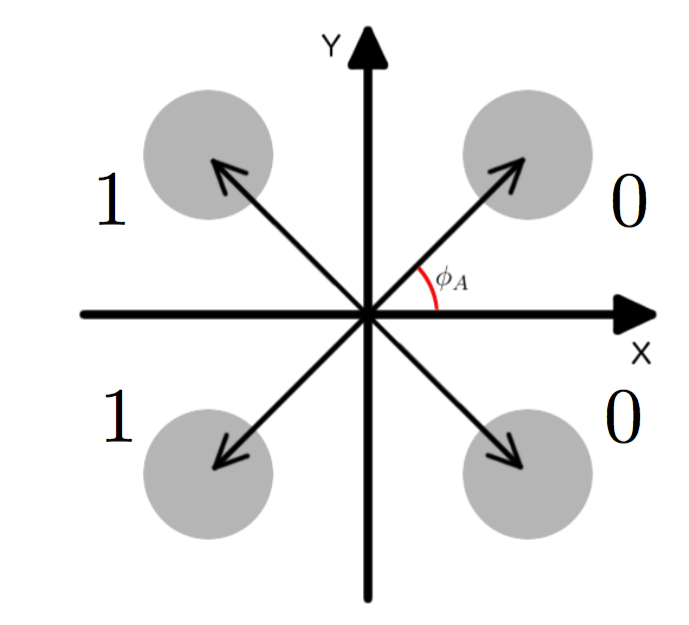
\includegraphics[width=.5\linewidth]{const.png}
	\caption{QPSK constellation.}
	\label{fig:constelacao}
\end{figure}

\bibliographystyle{unsrt}
\bibliography{bibliography}

\end{document}